\chapter{Sistemi di pagamento nella rete onion}
\label{cap:sistemi_di_pagamento}
La rete onion, come abbiamo visto, è fortemente basata sull'anonimato e sulla privacy. 
A differenza dei sistemi di pagamento tradizionali, che si basano su un sistema centralizzato e sulla forte identificazione\footnote{Le banche sono infatti obbligate a chiedere i documenti dei correntisti al fine di tenere traccia dei loro patrimoni e dei movimenti di denaro} degli utenti. 

\section{Bitcoin}
\label{sec:bitcoin}
BTC è la cripto valuta più utilizzata nella rete onion, alcuni report \cite{BTCdarkWeb} affermano che nei primi 4 mesi del 2020 il traffico di BTC nel dark web era di 795 milioni di dollari \footnote{Valore derivato dalla somma del traffico di denaro inviato e ricevuto da enti che operano nella rete TOR}, un aumento del 65\% rispetto allo stesso periodo del 2019.\\
Creata nel 2007 da Satoshi Nakamoto\footnote{Uno pseudonimo, la vera identità di Satoshi Nakamoto è ancora sconosciuta} è la prima cripto valuta decentralizzata, fu pensata come una moneta virtuale assente da un ente centrale che ne controllasse la circolazione e la creazione.\\
Il sistema di transazioni BTC è basato sulla \textit{blockchain}, un registro pubblico strutturato come una catena di blocchi, in cui ogni blocco rappresenta una transazione.
Ogni transazione contiene la chiave pubblica del proprietario, l'hash del blocco precedente, la chiave privata e la firma digitale del precedente proprietario. 
Questo impedisce di modificare la catena, in quanto questo cambierebbe l'hash e invaliderebbe i blocchi successivi.\\
Una domanda comune è: \textit{Come può un sistema basato su transazioni pubbliche essere usato in una rete basata sulla privacy?}, infatti chiunque può vedere le transazioni associate a un wallet semplicemente conoscendone l'indirizzo, non è però possibile risalire al proprietario perché nessun dato personale è associato all'indirizzo. 
Chi usa il proprio indirizzo nella rete TOR deve infatti stare attento a non associarlo alla sua persona, in quanto questo potrebbe essere usato per risalire alla sua identità. \cite{BTCcashSystem}

\section{Creazione di un wallet BTC}
Per accettare pagamenti nel nostro servizio onion abbiamo bisogno di possedere un indirizzo BTC. 
Ci sono wallet che possiamo usare per gestire i pagamenti, per questo esempio useremo Electrum\footnote{https://electrum.org/}, un wallet open source e gratuito.\\
una volta installato ed eseguito possiamo creare un nuovo wallet, scegliendo un nome, il tipo Standard Wallet, possiamo inoltre scegliere se usare un seed già esistente oppure generarne uno nuovo.\\
È inoltre importante salvare il seed in un luogo sicuro, in quanto questo è l'unico modo per recuperare il wallet in caso di perdita.
Da qui possiamo creare un nuovo indirizzo BTC, cliccando su \textit{Ricevi}, impostando la scadenza su Never e poi cliccando su \textit{Crea Richiesta}, successivamente cliccando su Bitcoin URI possiamo visualizzare il solo indirizzo BTC. 
\importImage{
    \label{fig:Electrum_ricevi} 
    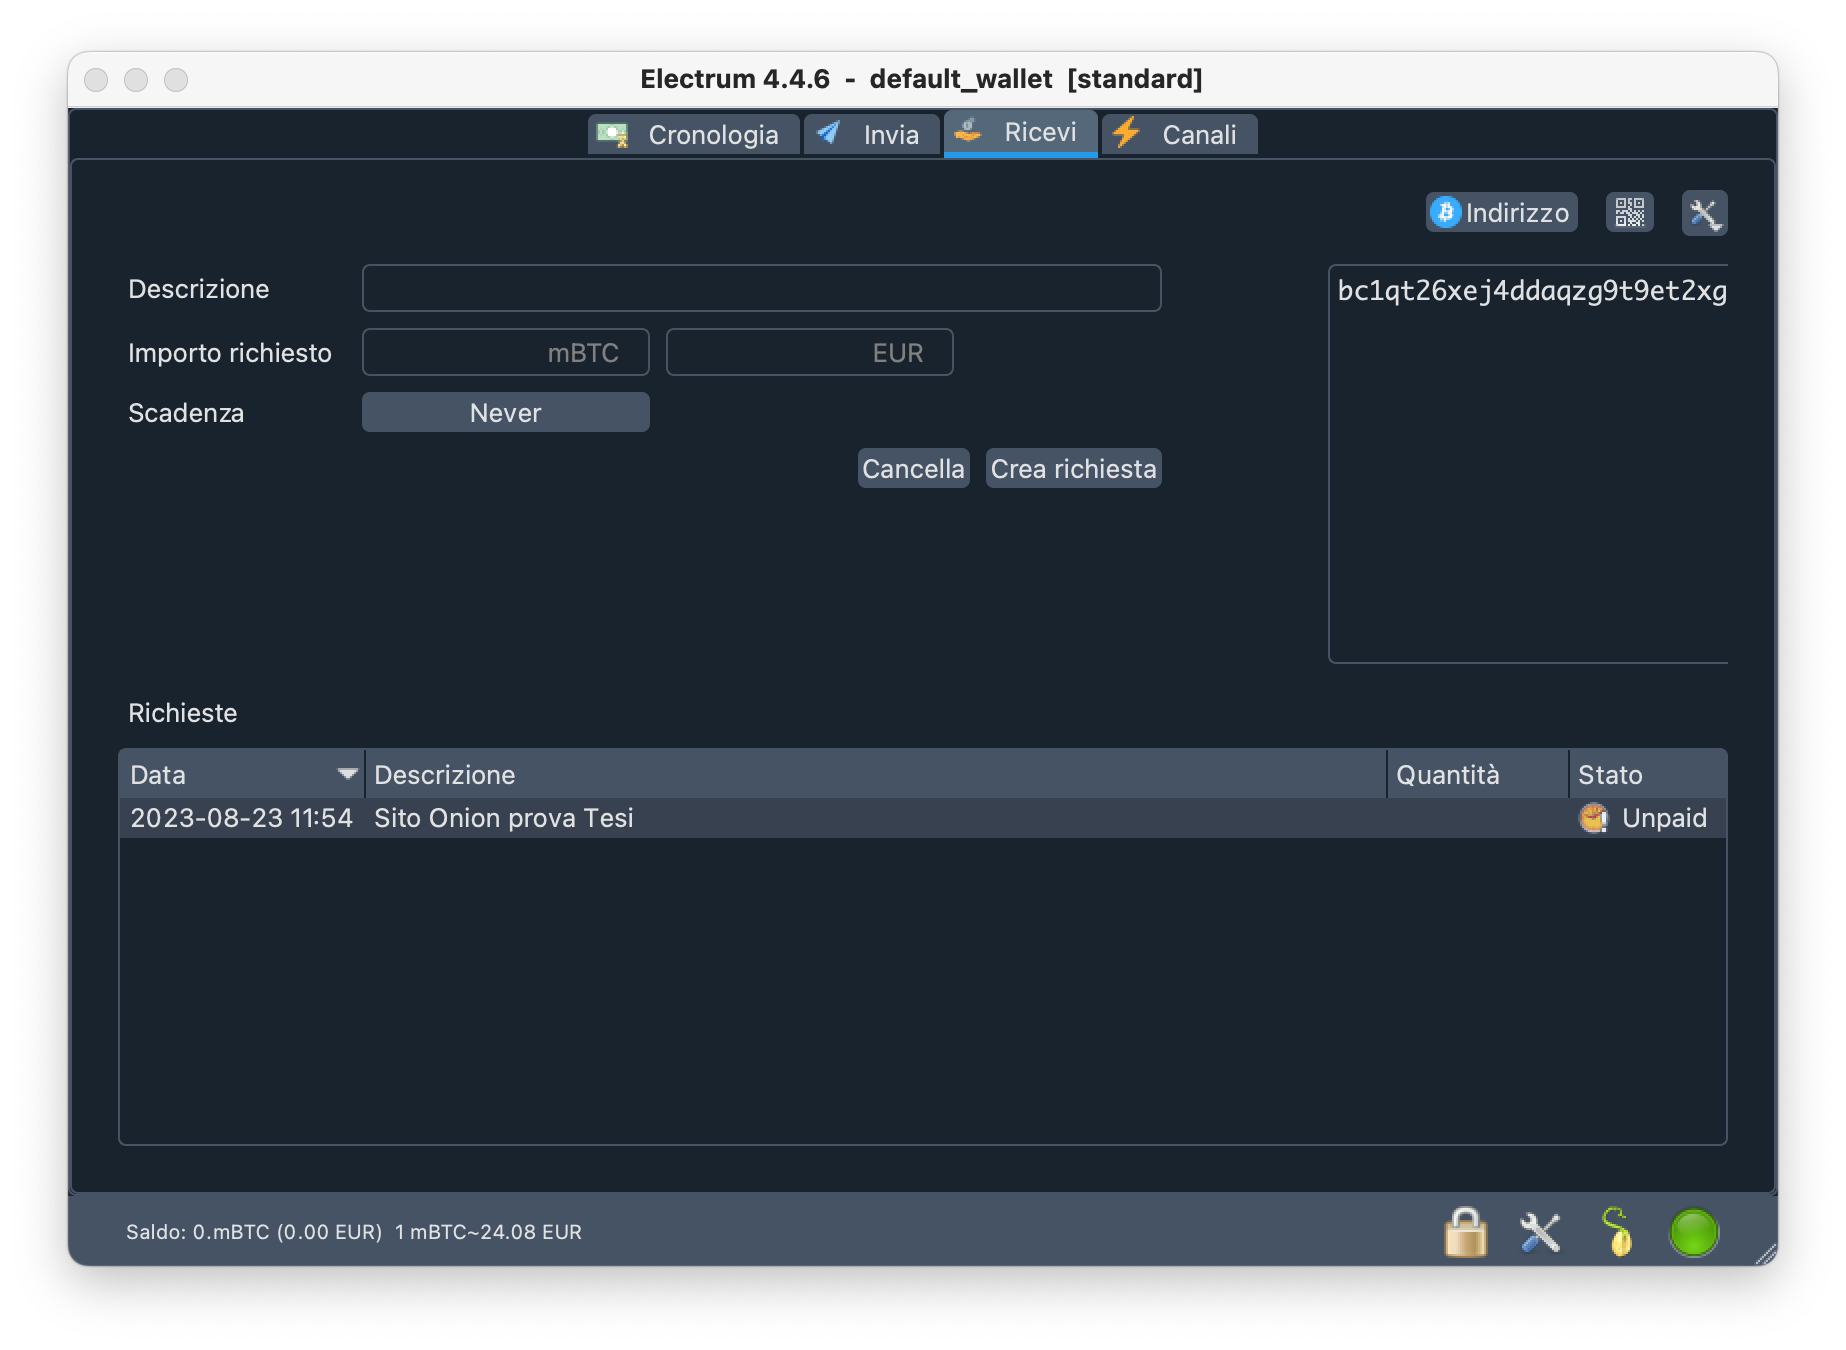
\includegraphics[width=0.75\textwidth]{Electrum/ricevi}
    \caption{Pagina ricevi con indirizzo BTC}
}\\
A questo punto possiamo copiare l'indirizzo e inserirlo nella pagina di pagamento del nostro servizio onion, oppure possiamo far generare un qrcode e inserirlo nella pagina.
\importImage{
    \label{fig:Electrum_ricevi_qr} 
    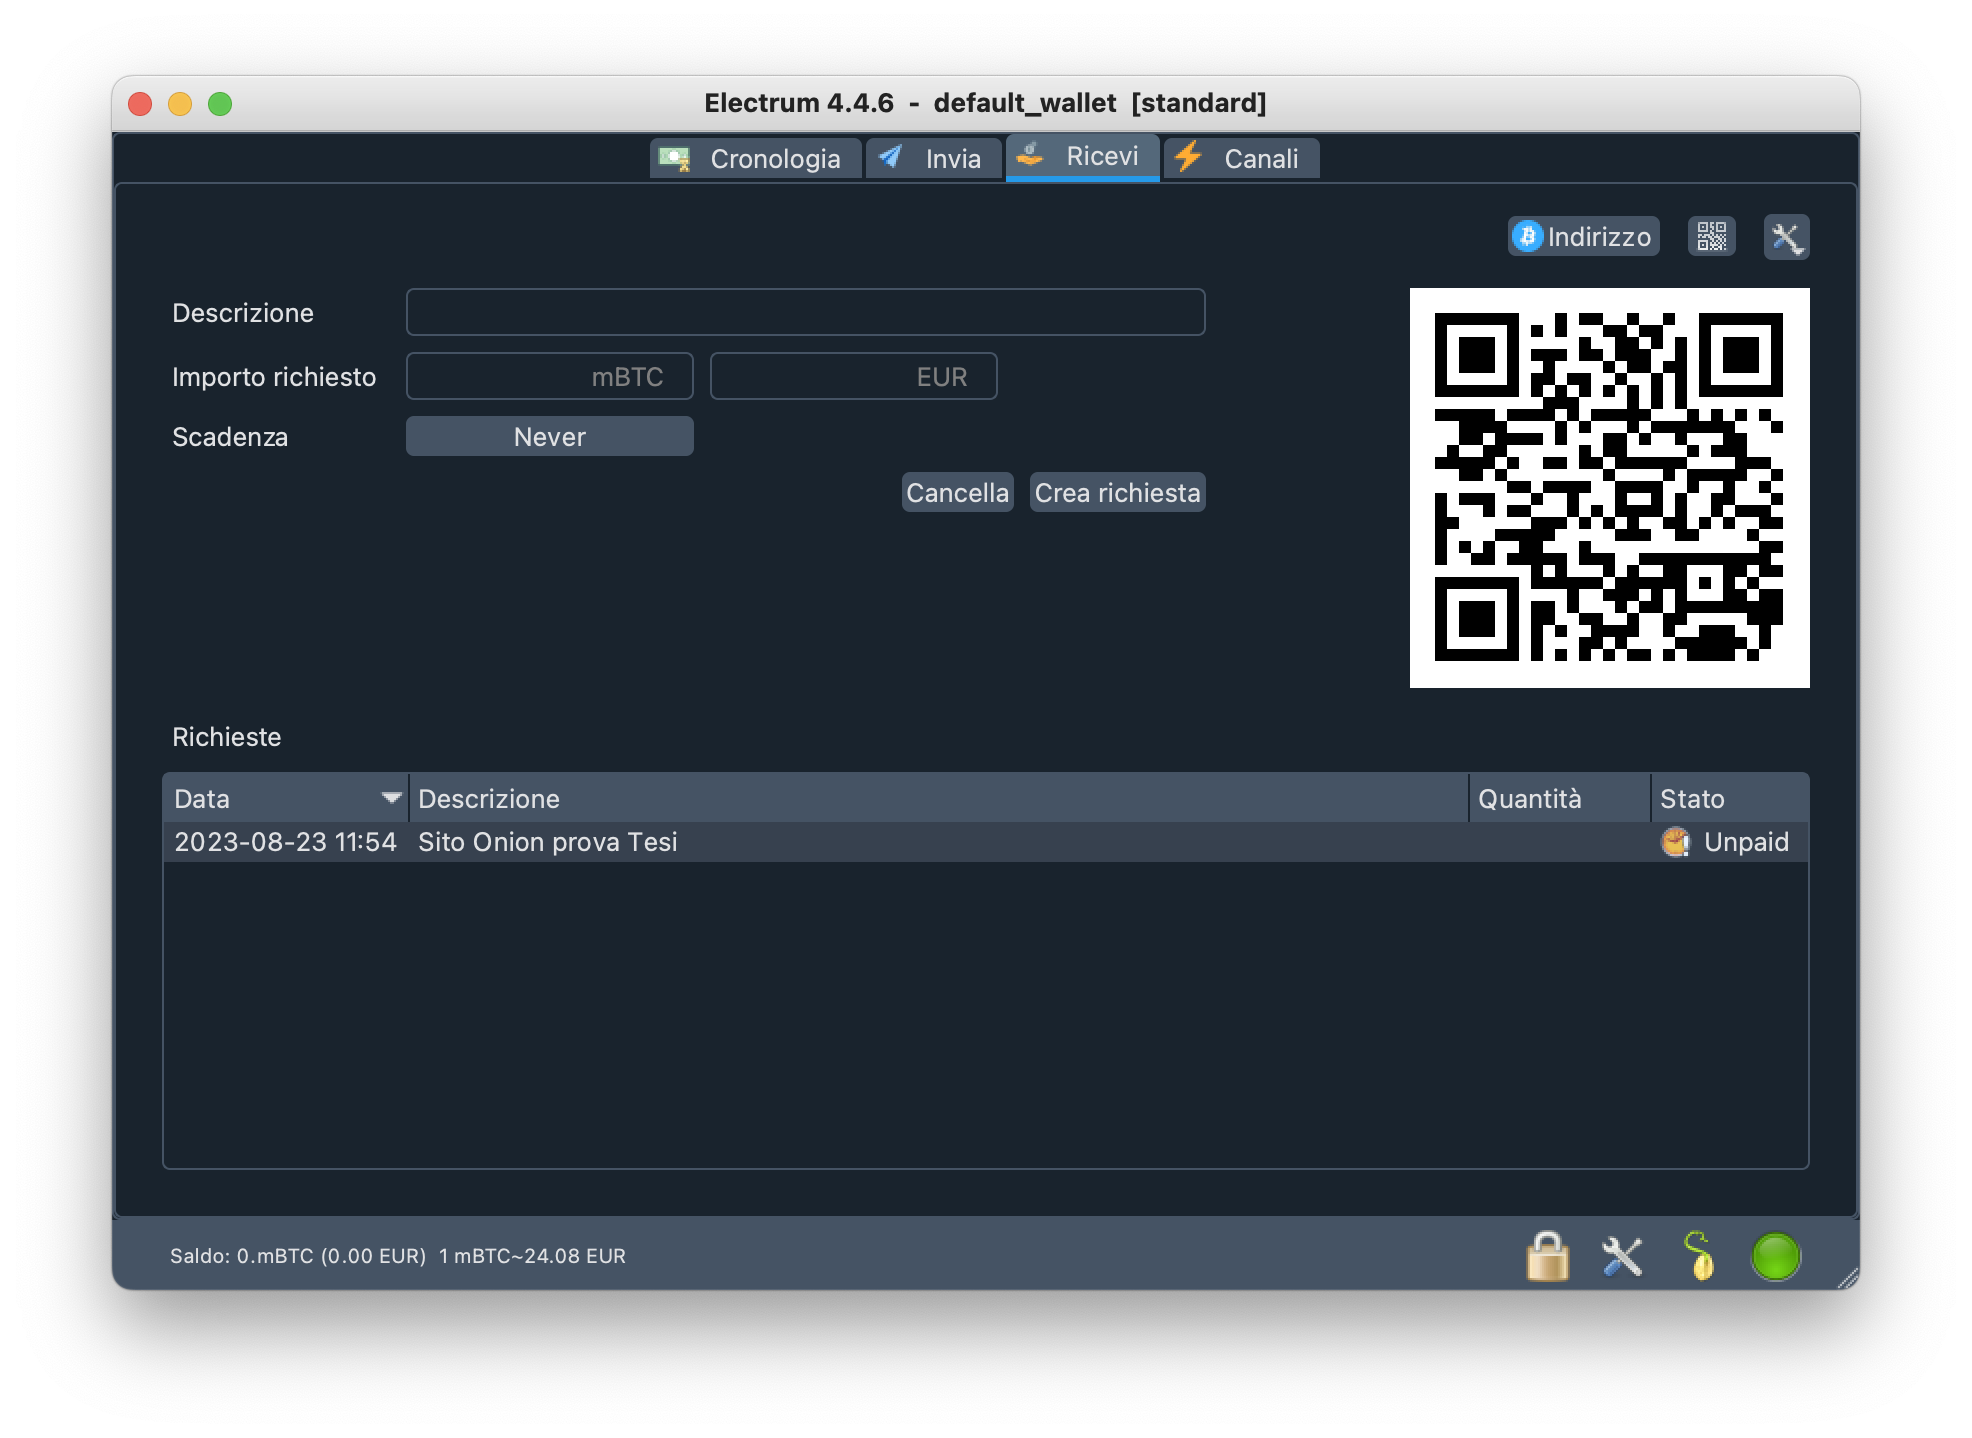
\includegraphics[width=0.75\textwidth]{Electrum/ricevi-qr}
    \caption{Pagina ricevi con qrcode}
}
